\chapter{Evaluation}
We evaluate our method based on the development data set from the ChAirGest
corpus~\cite{Ruffieux2013} with gestures captured from 10 users. There are
10 different gestures and 3 resting positions. There are 900 total gesture
occurrences (3 recording sessions for each user) in the development data set representing three forth of the entire corpus. The remaining one forth of the corpus are not released to
the public, and can be used for final evaluation on unseen data.

In this data set, on average, the hand is at 1.2m away
from the sensor, which means the depth error is around 5mm.

A frame-based accuracy score can be biased because a classifier that
favors longer gestures would have higher accuracy.

\textit{Precision} (P) corresponds to the number of correctly detected events
divided by the number of returned events and the \textit{Recall} metric
corresponds to the number of correctly detected events divided by the number of
events in the ground truth. \cite{Ruffieux2013}

\begin{align}
F1 = 2\times\frac{P \times R}{P + R}
\end{align}

\begin{table}[h]
\begin{center}
\begin{tabular}{|l|p{2cm}|p{1.7cm}|p{1.7cm}|}
\hline
 & Hand position from salience detection \& Xsens & Hand position
 from Kinect skeleton \& Xsens & Xsens Only \\
\hline
F1 Score & \textbf{0.907 (0.01)} & 0.870 (0.02) & 0.890 (0.02) \\
\hline
ATSR Score & \textbf{0.923 (0.02)} & 0.930 (0.03) & 0.920 (0.01) \\
\hline
Final Score & \textbf{0.912 (0.01)} & 0.881 (0.01) & 0.895 (0.01) \\
\hline
\end{tabular}
\caption{Comparison of the average 3-fold cross validation results for different
feature vectors. Values in parentheses are standard deviations.}
\label{tab:comp-feature}
\end{center}
\end{table}

If we only use motion features such as relative position, velocity and
acceleration, the result is poor because it cannot distinguish gestures with
the same path but different hand postures such as ``Wave Hello'' and ``Shake
Hand'', ``Circle Palm Rotation'' and ``Circle Palm Down''.

\begin{table}[h]
\begin{center}
\begin{tabular}{|l|p{2cm}|p{2cm}|p{1.7cm}|p{1.7cm}|}
\hline
          & motion & color & depth & both \\
\hline
F1 Score & 0.677 (0.04) & 0.703 (0.01) & 0.720 (0.02) & 0.723 (0.01) \\
\hline
ATSR Score & 0.893 (0.02) & 0.870 (0.01) & 0.880 (0.01) & 0.873 (0.01) \\
\hline
Final Score & 0.710 (0.03) & 0.732 (0.01) & 0.748 (0.01) & 0.749 (0.00) \\
\hline
\end{tabular}
\caption{Comparison of the average 3-fold cross validation results for
features from color and depth sensors. Values in parentheses are standard
deviations.}
\label{tab:comp-feature}
\end{center}
\end{table}

\begin{figure}[h]
\centering
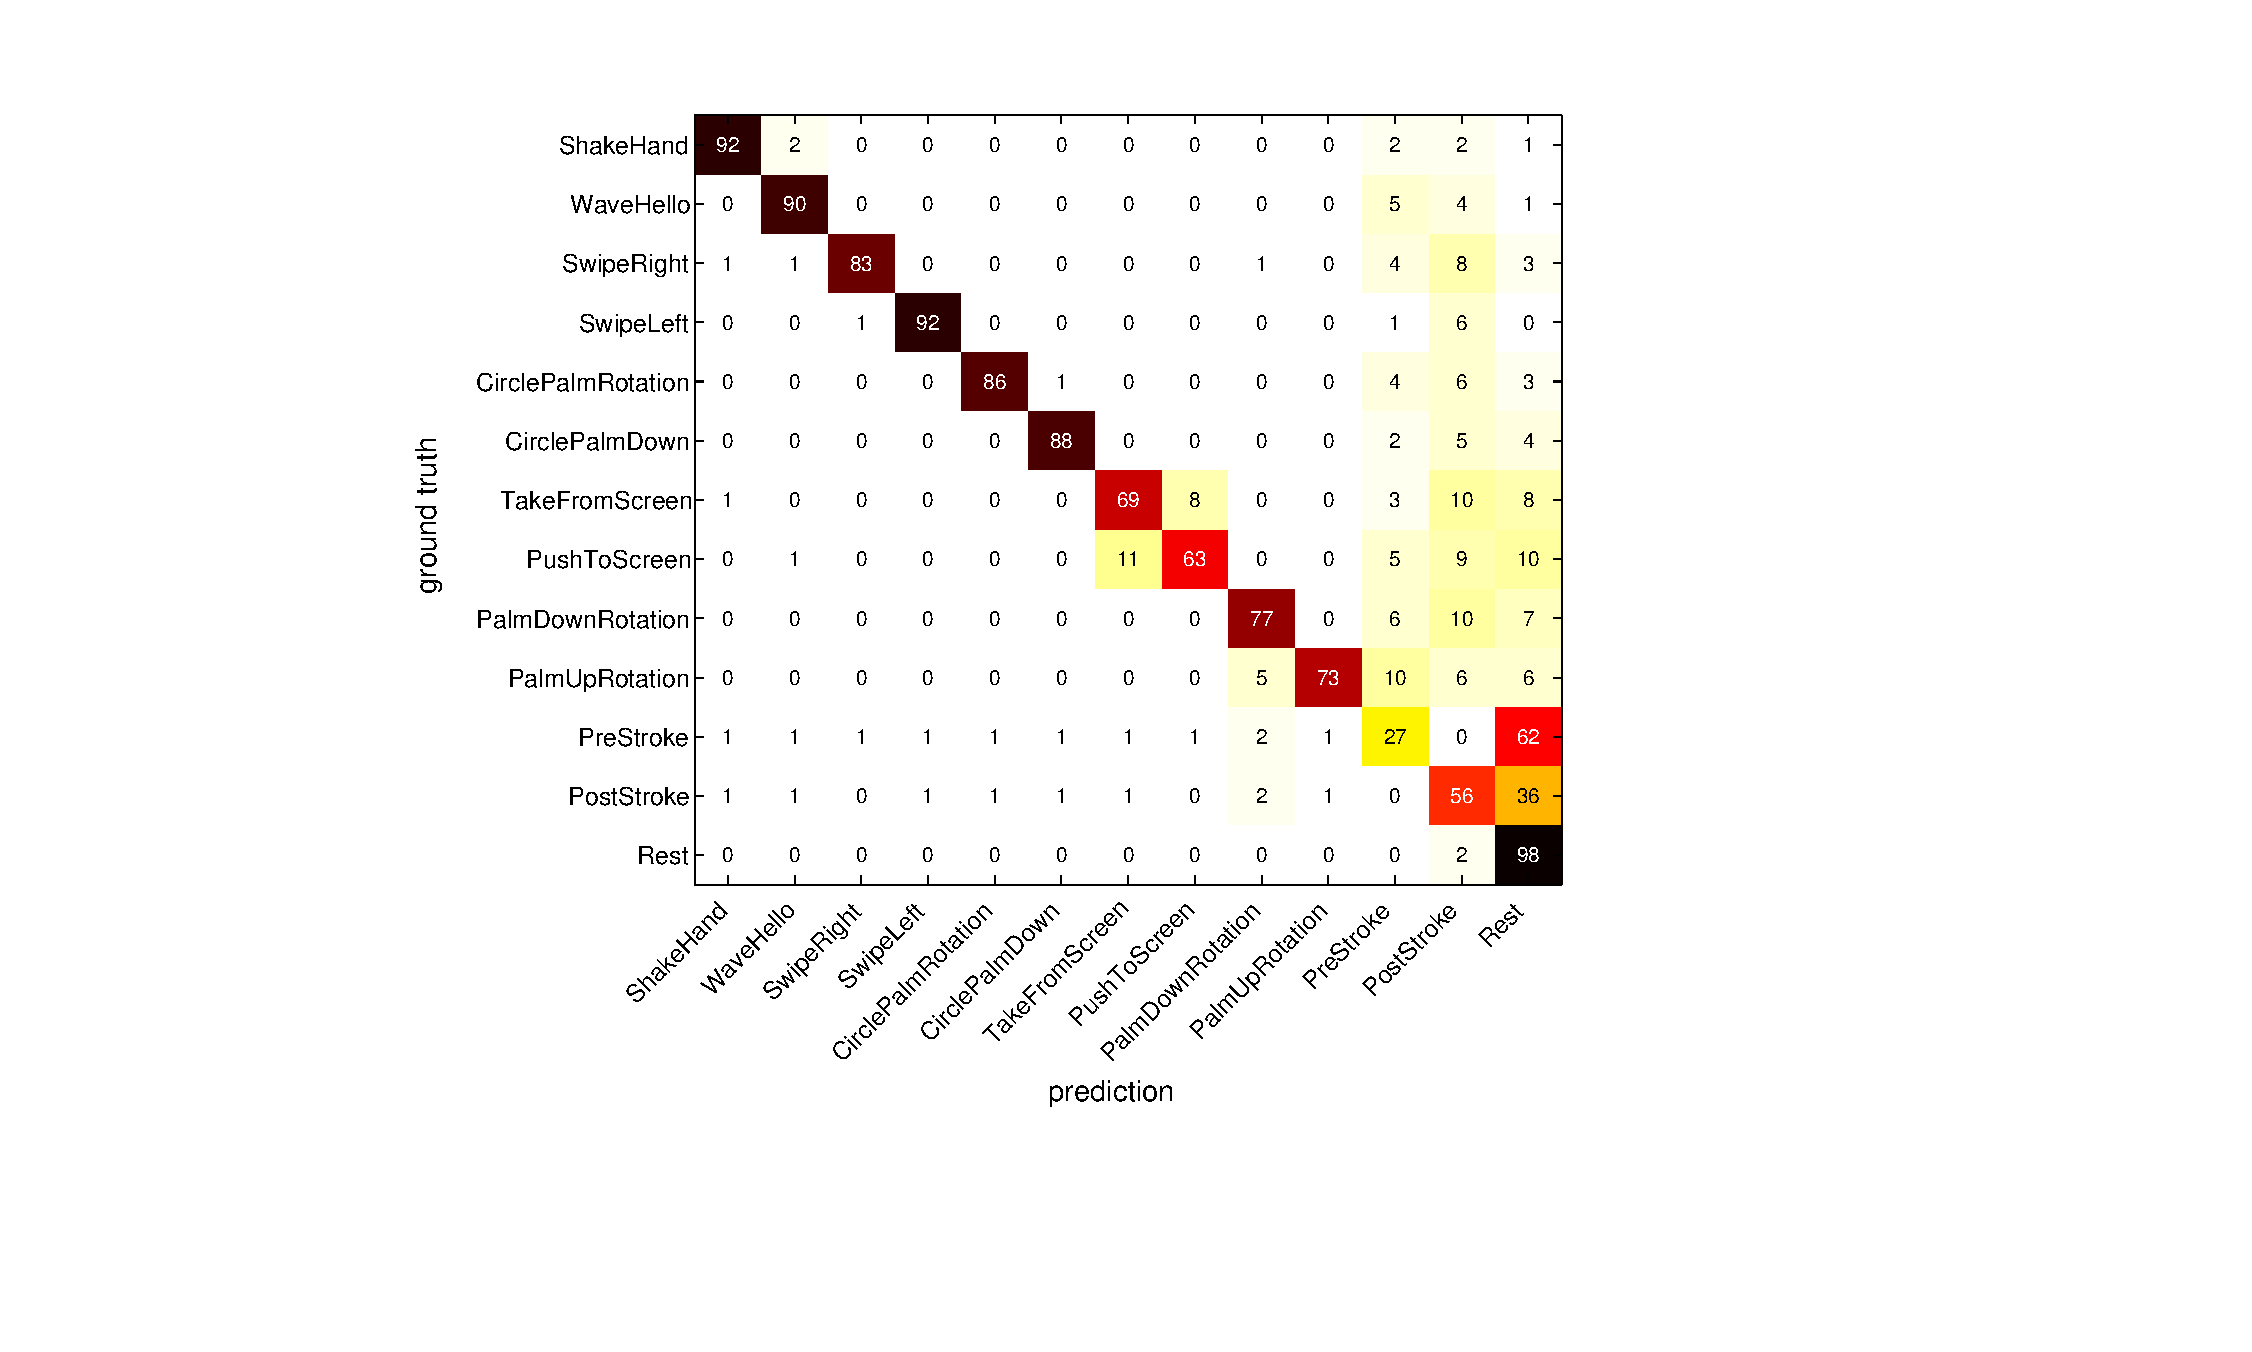
\includegraphics[trim={6cm 3.5cm 10cm 1.5cm}, clip,
width=0.5\columnwidth]{figures/confusion-matrix.eps} \caption{Per frame
classification confusion matrix based on result from 3-fold cross validation using both Kinect and Xsens features. The numbers are percentages. The darker the color the higher the percentage.}
\label{fig:confusion}
\end{figure}

\begin{figure}[h]
\centering
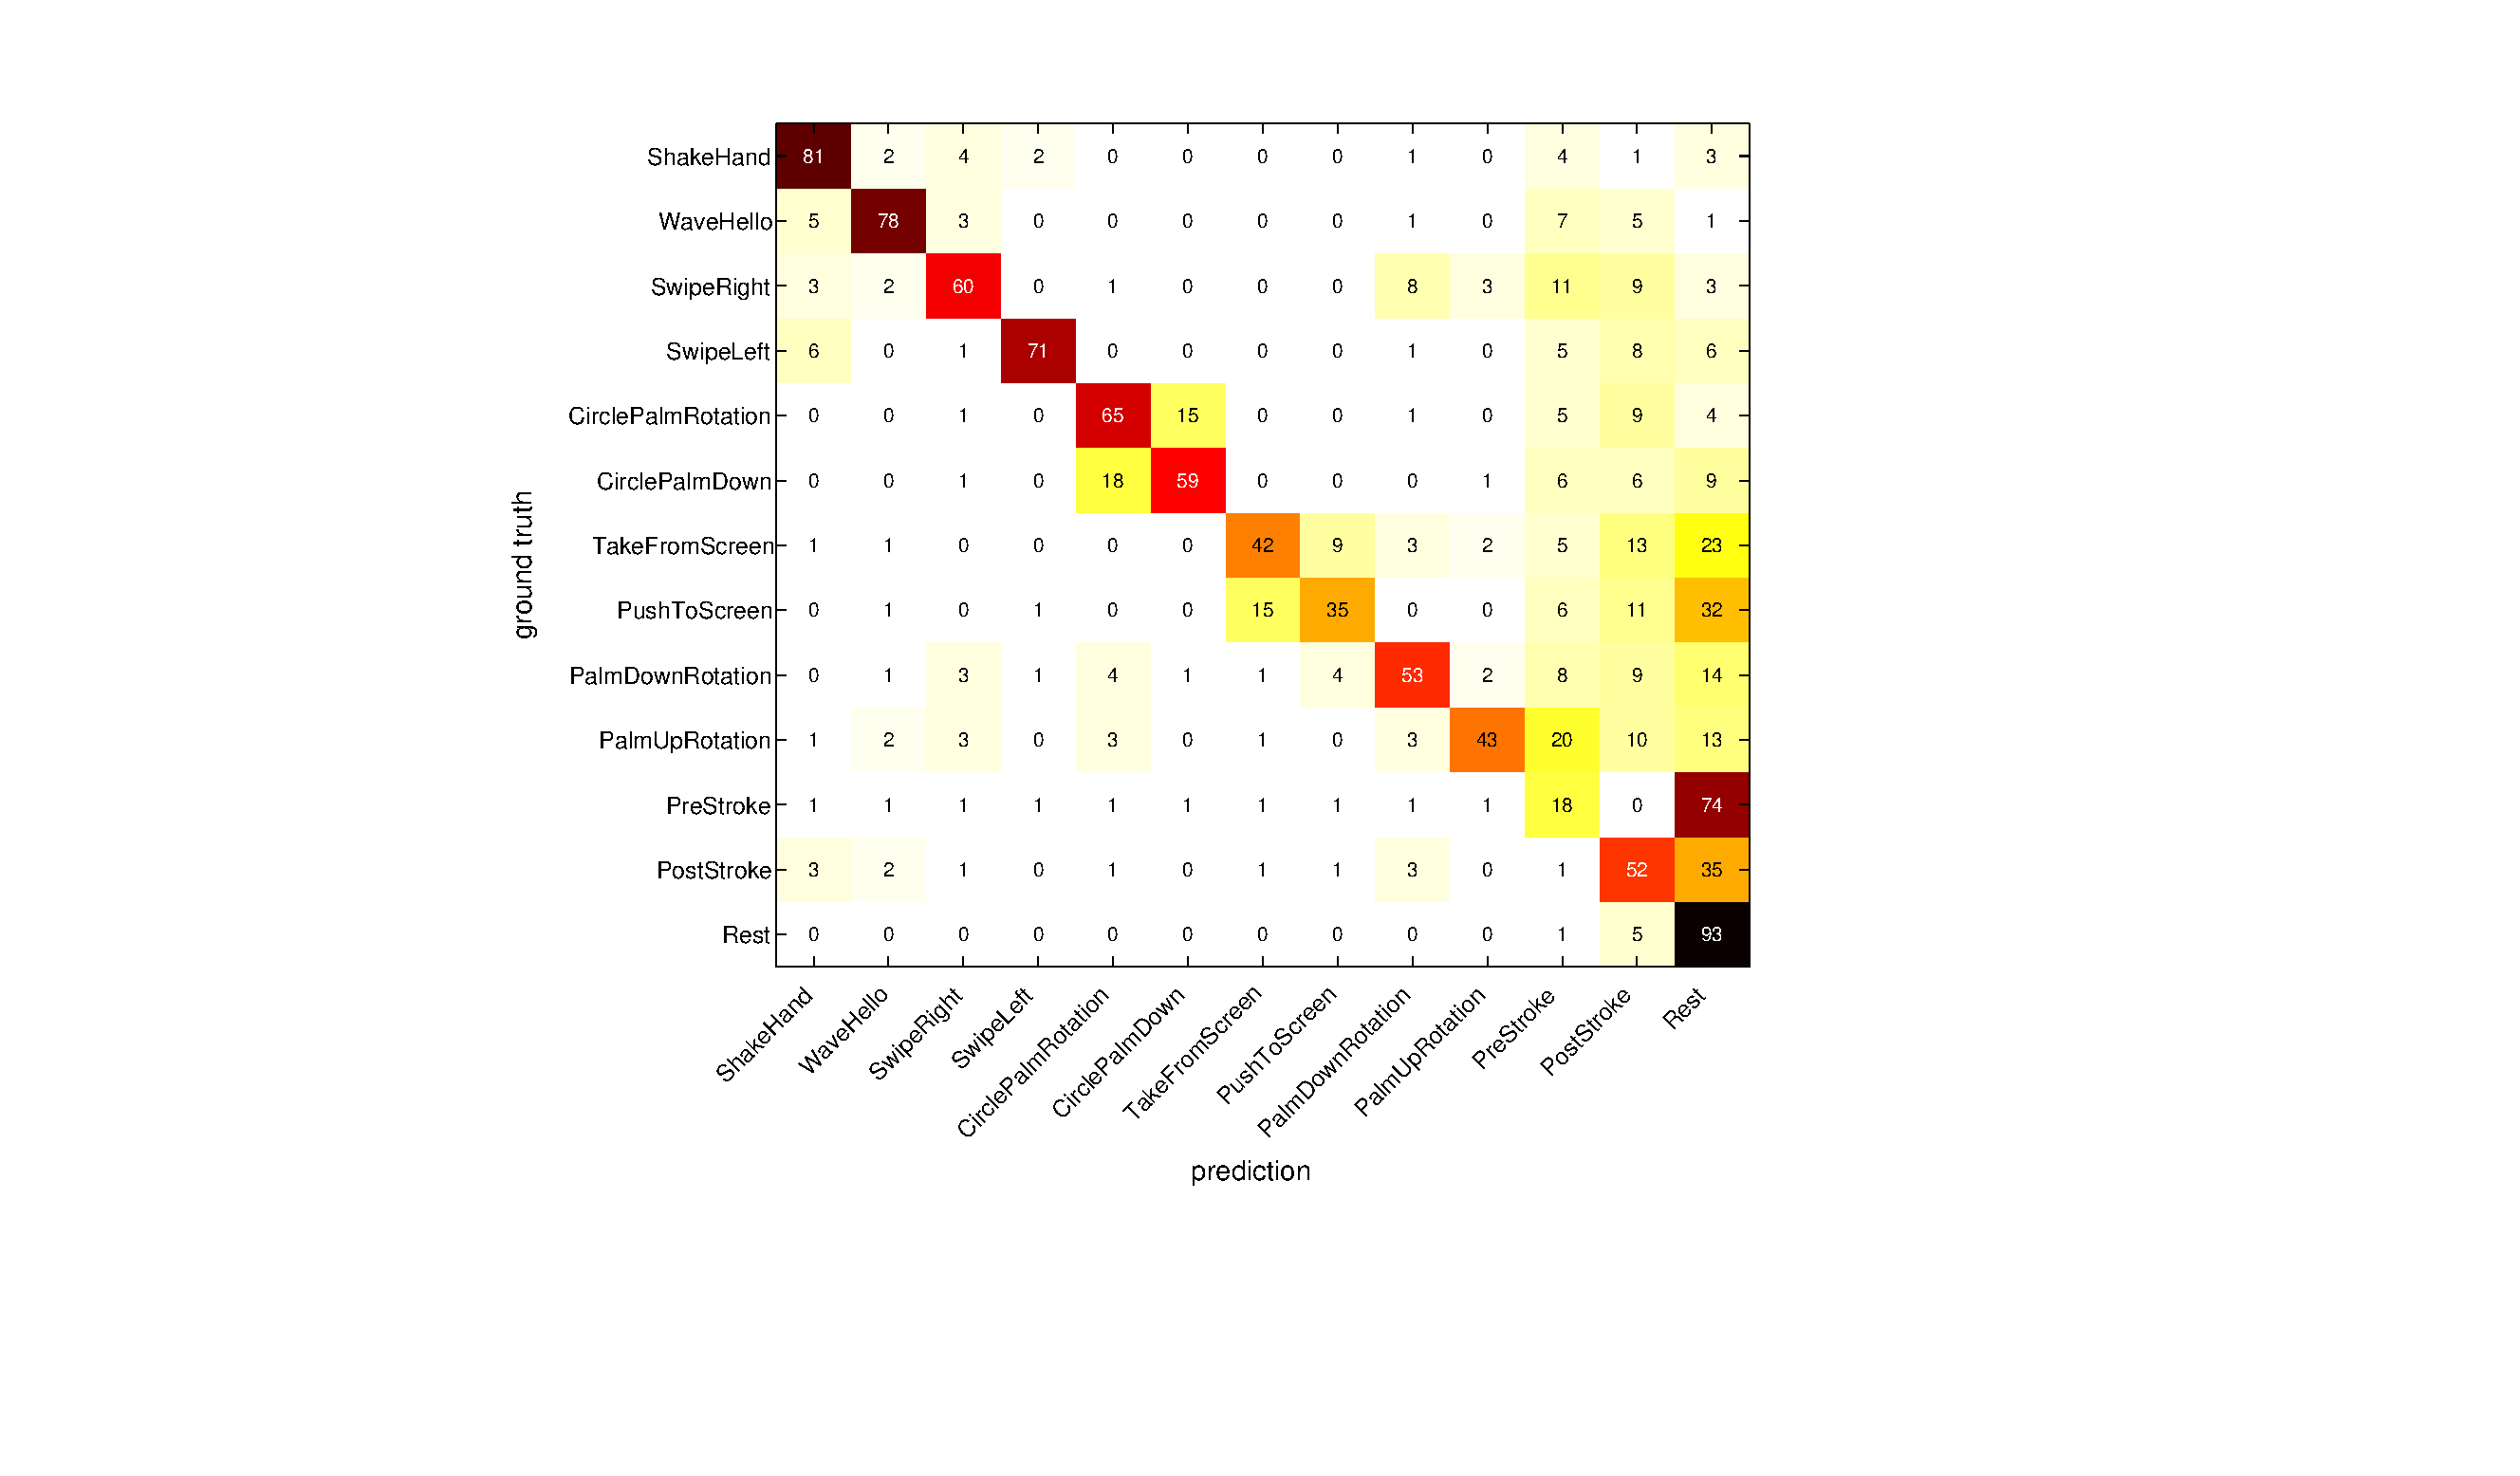
\includegraphics[trim={6cm 3.5cm 10cm 1.5cm}, clip,
width=0.6\columnwidth]{figures/confusion_motion.eps} \caption{Per frame
classification confusion matrix based on result from 3-fold cross validation
using motion features only (relative position, velociy, acceleration). The
numbers are percentages.
The darker the color the higher the percentage.}
\label{fig:confusion}
\end{figure}

\begin{figure}[tb]
\centering
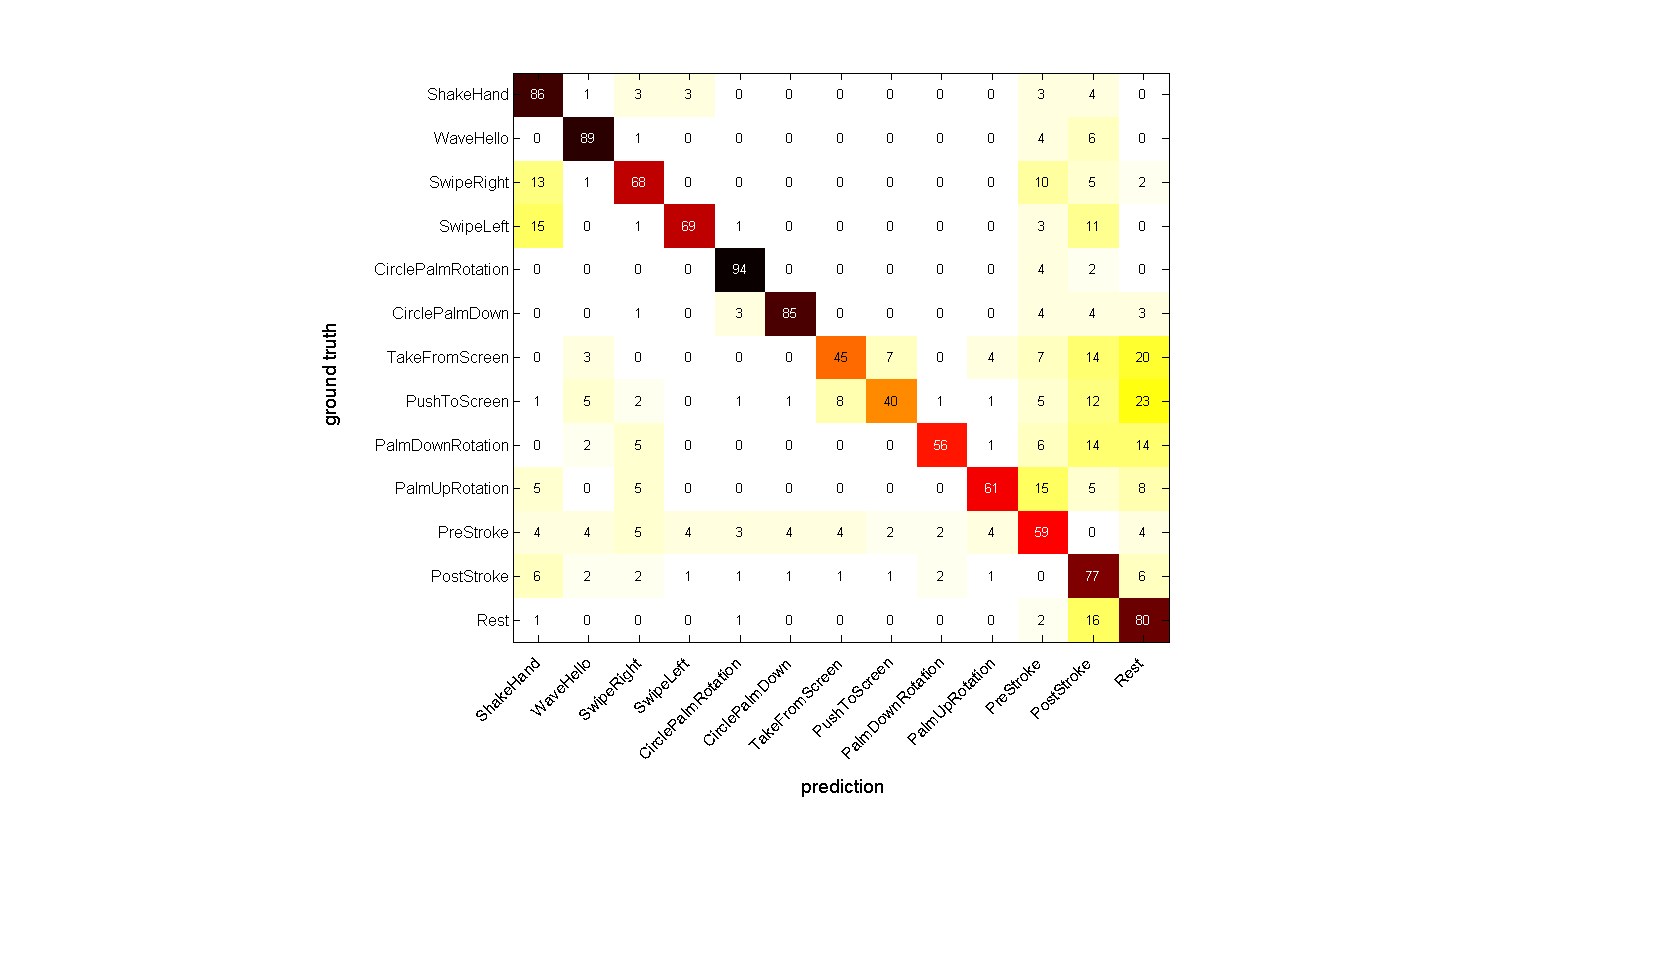
\includegraphics[trim={6cm 3.5cm 10cm 1.5cm}, clip,
width=0.6\columnwidth]{figures/confusion_color_depth.png} \caption{Per frame
classification confusion matrix based on result from 3-fold cross validation using 
both color and depth images for hand. The numbers are percentages. The darker
the color the higher the percentage.}
\label{fig:confusion}
\end{figure}

``Take from Screen'' and ``Push to Screen'' have the lowest recognition
accuracy, especially when using the kienct data. We notice that when the users
extend their hands towards the screen, the hands are too close to the sensor
(below the too near range), and the depth sensor cannot get accurate readings.

We evaluate our method based on the dataset we collected, using the
evaluation metrics proposed in the previous section. The evaluation is based
on the assumption that all the gestures with distinct paths (gesture \#1--4)
are discrete flow gestures, and gestures with distinct hand poses (gesture
\#5--7) are continuous flow gestures. 

Our survey results show that it is
important to allow users to quickly define and train their own gestures. Hence,
we evaluate our system using user dependent training and testing. For each user
in the dataset, we use the first 2 sessions of recording (6 samples per gesture)
as training examples, and the last 2 sessions as testing examples.
Fig.~\ref{fig:recog-result} shows a visualization of the recognition result on a
test sequence. The figure highlights the challenges in the test sequences:
there are 21 gestures in each continuous unsegmented sequence; sometimes
gestures immediately follow one another.

We report the average results for 10 users.

\begin{figure}[t]
\centering
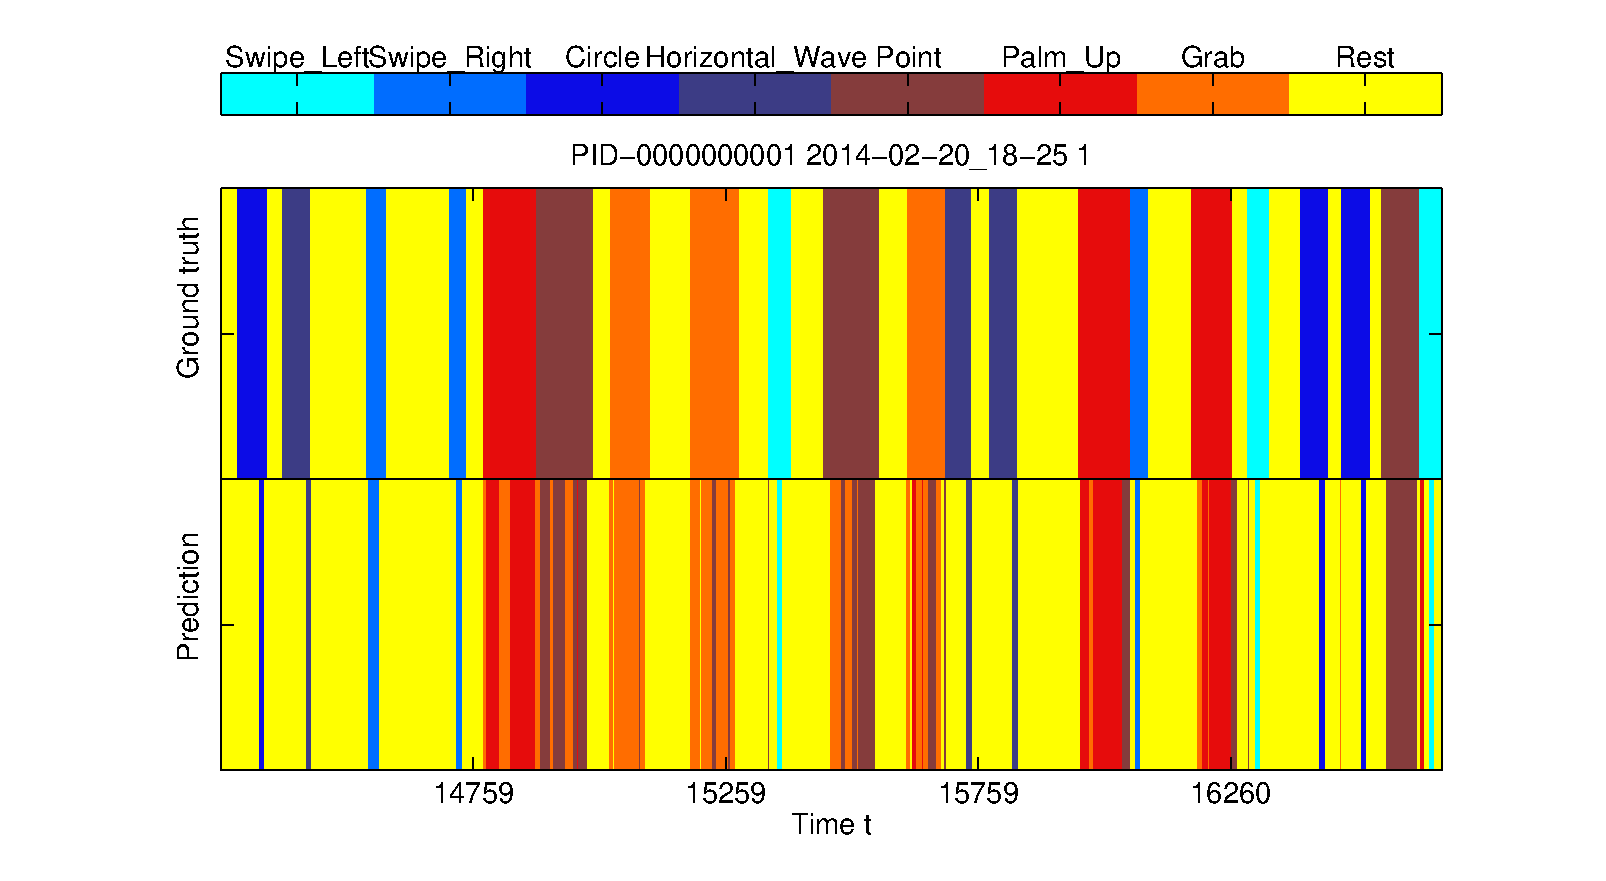
\includegraphics[trim=10mm 5mm 10mm 5mm, clip,
width=\columnwidth]{fig/recog_result_m3.eps}
\caption{Comparison between recognition result using online inference
and ground truth.
The colors correspond to different gestures. For discrete flow gestures
(swipe left/right, circle, horizontal wave), one color segment with a fixed
length is shown at the time of response. For continuous flow gestures, the
recognized gesture is shown at each frame indicating frame-by-frame responses.}
\label{fig:recog-result}
\end{figure}

\section{Compare Different Topologies}
In our unified framework, is it necessary to
treat gestures with distinct hand poses differently from gestures with
distinct paths? Table~\ref{tab:result} compares the results between two topologies. The first
row is the result from treating the two forms of gestures in the same way,
i.e., all gestures have the same left-right Bakis model for their nucleus
phases. The second row is the result from using a left-right Bakis model for
gestures with distinct paths and a single state for gestures with distinct hand
poses.
As Table~\ref{tab:result} shows, having different HMM topologies for the two forms of gestures significantly increases the precision, recall and F1 score for gestures with
distinct hand poses.

For gestures with arbitrary movement, it is difficult to use embedded training
to accurately align pre-stroke, nucleus and post-stroke phases.
Figure~\ref{fig:palm-hidden} illustrates this problem. It shows the most likely
hidden state estimates for a ``palm up'' gesture sequence. The main (center)
part of the gesture is identified as the post-stroke of the gesture.

\begin{figure}
\centering
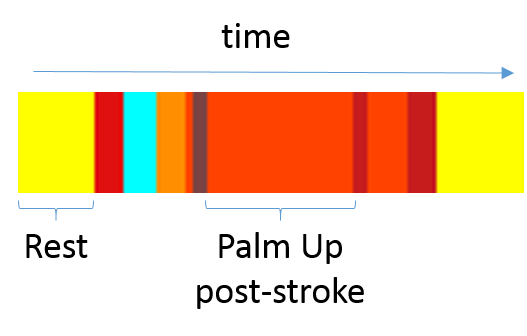
\includegraphics[width=0.3\linewidth]{figures/palm_hidden_label.png}
\caption{Estimated hidden states for a ``palm up'' gesture using the left-right
model same as gestures with distinct path. Different colors correspond to
different hidden states.}
\label{fig:palm-hidden}
\end{figure}

\begin{table}[t]
\caption{Results from using different topologies. The numbers in parentheses are
standard deviations. The results are based on using 3 mixtures of Gaussians
for the emission probabilities, and lag time $L = 8$ frames.}
\label{tab:result}
\centering
\begin{tabular}{|l|l|p{3cm}|p{3cm}|}
\hline
& & Same topology for two forms of gestures & Different topologies for two forms
of gestures \\
\hline
\multirow{4}{4cm}{Distinct paths \& discrete flow gestures} 
& Precision & 0.84 (0.16) & 0.83 (0.13) \\
\cline{2-4}
& Recall & 0.87 (0.17) & 0.87 (0.16)\\
\cline{2-4}
& F1 & 0.85 (0.16) &  0.85 (0.13)\\
\cline{2-4}
& Responsiveness (s) & 0.6 (0.3) & 0.7 (0.3) \\
\hline
\multirow{4}{4.5cm}{Distinct hand poses \& continuous flow gestures}
& Precision & 0.65 (0.14) & 0.57 (0.09) \\
\cline{2-4}
& Recall & 0.41 (0.15) & 0.65 (0.08) \\
\cline{2-4}
& F1 & 0.50 (0.14) & 0.61 (0.09) \\
\hline
\textbf{Average} & F1 & 0.675 (0.15) & \textbf{0.72 (0.11)} \\
\hline
\end{tabular}
\end{table}

\section{Compare different number of mixtures}
Within a user, there may be variation in the hand pose for a
gesture with distinct hand pose. For example, the ``point'' hand pose can have
different orientations. This is why we use a mixture of Gaussians for the
emission probabilities. Fig.~\ref{fig:mixtures}
shows that the F1 scores increases as the number of mixtures (M) increases until $M=3$.
After that, we start to see the effect of overfitting.

\begin{figure}[t]
\centering
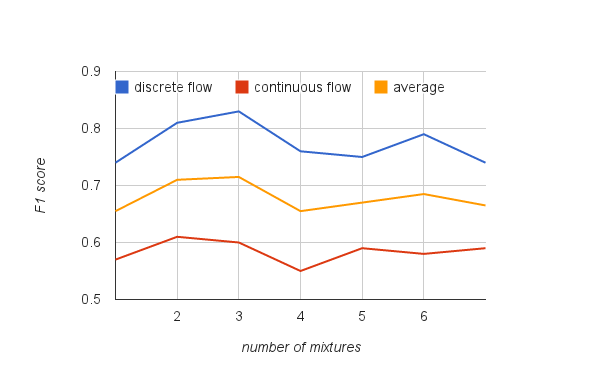
\includegraphics[trim=10mm 5mm 10mm 15mm,
clip, width=\columnwidth]{figures/f1_nM.png}
\caption{F1 scores versus number of mixtures.}
\label{fig:mixtures}
\end{figure}

%Compare user dependent vs user independent result

\section{Compare Different Lag Times}
Fig.\ref{fig:lag} shows how the F1 scores change with respect to the lag time
($L$) in fixed-lag smoothing. The performance increases as $L$ increases, and
plateaus at $L=8$ frames which is about 0.3s at 30 FPS. This shows that more
evidence does help to smooth the estimates until a limit, and we do not need to
sacrifice too much delay to reach the limit. Our result also shows that the
responsiveness score stays around 0.6-0.7 seconds as we increase $L$.

\begin{figure}[t]
\centering
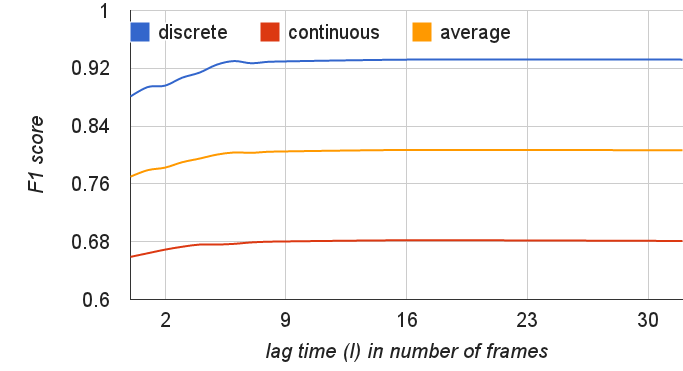
\includegraphics[trim=0 5mm 0 15mm, clip,
width=\columnwidth]{figures/f1_lag.png}
\caption{F1 scores versus lag time.}
\label{fig:lag}
\end{figure}

Our system is fast to train as well. The average computation time for training
the model for one user is about 5s with 7 gestures and 6 training examples per
gesture.